\documentclass[a4paper, 11pt]{article}
\usepackage{amsmath}
\usepackage{graphicx}
\usepackage{geometry}
\usepackage{listings}
\usepackage{xcolor}
\usepackage[colorlinks,linkcolor=red]{hyperref}
\geometry{scale=0.8}

\title{	
\normalfont \normalsize
\textsc{School of Data and Computer Science, Sun Yat-sen University} \\ [25pt] %textsc small capital letters
\rule{\textwidth}{0.5pt} \\[0.4cm] % Thin top horizontal rule
\huge  E01 Maze Problem\\ % The assignment title
\rule{\textwidth}{2pt} \\[0.5cm] % Thick bottom horizontal rule
\author{18340052   何泽}
\date{\normalsize\today}
}

\usepackage[UTF8]{ctex}
\begin{document}
\maketitle
\tableofcontents
\newpage
\section{Task}



\begin{itemize}
	\item Please solve the maze problem (i.e., find the shortest path from the start point to the finish point) by using BFS or DFS (Python or C++)
	\item The maze layout can be modeled as an array, and you can use the data file \texttt{MazeData.txt} if necessary.
	\item Please send \texttt{E01\_YourNumber.pdf} to \texttt{ai\_2020@foxmail.com}, you can certainly use \texttt{E01\_Maze.tex} as the \LaTeX template.
\end{itemize}

\begin{figure}[ht]
\centering
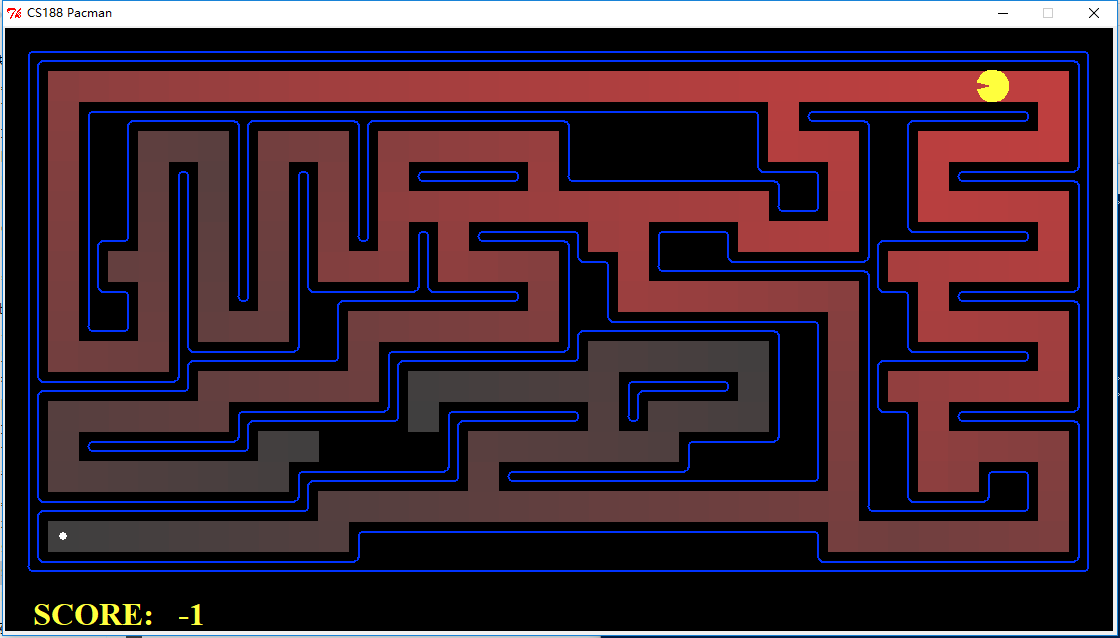
\includegraphics[width=15cm]{Pic/Pacman}

\caption{Searching by BFS or DFS}
\end{figure}


\section{Codes}
\lstset{
	columns=fixed,       
	numbers=left,                                        % 在左侧显示行号
	frame=shadowbox,                                          % 不显示背景边框
	backgroundcolor=\color[RGB]{245,245,244},            % 设定背景颜色
	keywordstyle=\color[RGB]{0,92,230},                 % 设定关键字颜色
	numberstyle=\footnotesize\color{darkgray},           % 设定行号格式
	commentstyle=\it\color[RGB]{0,96,96},                % 设置代码注释的格式
	stringstyle=\rmfamily\slshape\color[RGB]{230,92,0},   % 设置字符串格式
	showstringspaces=false,                              % 不显示字符串中的空格
	breaklines,
	language=Python,      
}
\begin{lstlisting}
def DFS(map, x, y, used):
	global res
	if len(res) and len(used) > len(res):
		return
	if x == -1 or y == -1 or x == len(map) or y == len(map[0]) or map[x][y] == '1' or (x, y) in used:
		return
	elif map[x][y] == 'E':
		print('\033[1;30;46m %d \033[0m' % (len(used) + 1), end="")
	if len(used) + 1 < len(res) or len(res) == 0:
		res = used
		res.append((x, y))
		return
	else:
		used.append((x, y))
		DFS(map, x + 1, y, used[:])
		DFS(map, x - 1, y, used[:])
		DFS(map, x, y + 1, used[:])
		DFS(map, x, y - 1, used[:])
	used.remove(used[-1])


def print_result(map, path):
	print(' ')
	print('\033[1;30;46m                   最短路径长度: %d                   \033[0m' % len(path))
	print('图示:')
	for i in range(len(map)):
		for j in range(len(map[i])):
			if (i, j) in path[1:-1]:
				print('\033[1;32;43m  \033[0m', end="")
			elif map[i][j] == "1":
				print('\033[1;33;44m  \033[0m', end="")
			elif map[i][j] == "S":
				print('\033[1;30;41mS \033[0m', end="")
			elif map[i][j] == "E":
				print('\033[1;30;45mE \033[0m', end="")
			else:
				print("  ", end="")
		print("")
	print("")


if __name__ == "__main__":
	print('\033[1;30;46m          何泽-18340052-人工智能实验一:Maze            \033[0m')
	print('\033[1;30;44m  蓝色是墙  \033[0m', end="")
	print('\033[1;30;41m  红色是起始点  \033[0m', end="")
	print('\033[1;30;45m  紫色是终点  \033[0m', end="")
	print('\033[1;30;43m  黄色是最短路径  \033[0m')
	print('\033[1;30;46m  历史路径长度:  \033[0m', end="")
	Maze = []
	res = []
	with open("./MazeData.txt", 'r') as Maze_og:
		for i in Maze_og.readlines():
			if i[0] == '1' or i[0] == '0':
		Maze.append(i[:-1])

	for i in range(len(Maze)):
		for j in range(len(Maze[i])):
			if Maze[i][j] == 'S':
				DFS(Maze, i, j, [])
				break

	print_result(Maze, res)
\end{lstlisting}
\section{Results}
\begin{figure}[!h]
\centering
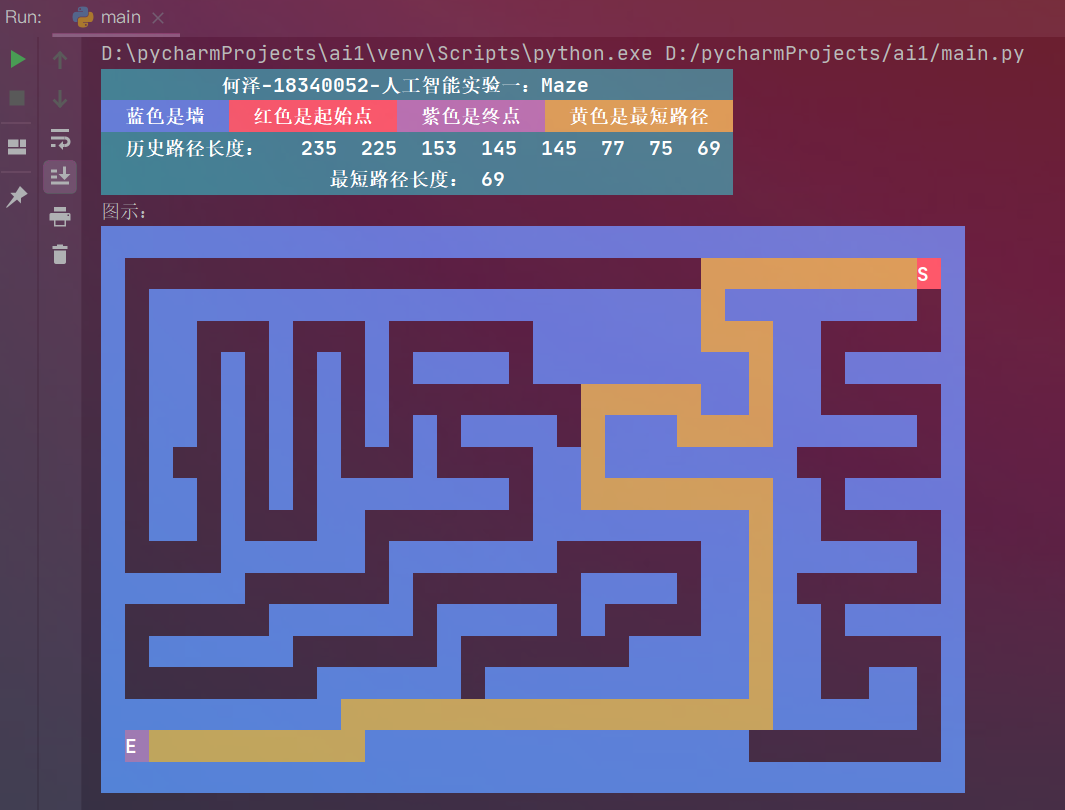
\includegraphics[width=13cm]{result.png}

\caption{Result}
\end{figure}
\begin{itemize}
	\item 首先说明了迷宫各种颜色的含义
	\item 我的算法采用了深度优先搜索
	\item 每找到一条路径,就会记录下来当前路径长度并打印,并给出最短路径长度
	\item 在图示中用色块画出了迷宫和最短路径,可以看出找出的路径确实是最短的
\end{itemize}

%\clearpage
%\bibliography{E:/Papers/LiuLab}
%\bibliographystyle{apalike}
\end{document} 